\subsubsection{Modelo económico}
\label{sec:economic-model}

A continuación se presenta el modelo económico, cuyos valores se expresan en dólares estadounidenses (USD). 
Sus parámetros se organizan en cuatro grupos. En primer lugar, los supuestos sobre gemas establecen que 
el creador retiene el 10\% de cada venta cosmética, y que la conversión es de \$0{,}25 por gema. En cuanto 
a las suscripciones, el precio por zona es de \$5{,}00 mensuales, con un costo de mantenimiento estimado de 
\$3{,}75 por zona. El costo de \$3{,}75 por zona, se base en que por maquina virtual se alojan 4 zonas, y cada máquina 
virtual tiene un costo mensual de \$15{,}00, mas detalles en la seccion de \nameref{sec:load-test}.

\vspace{0.25cm}

Respecto a las comisiones de Stripe, se aplica una tarifa variable del 2{,}90\% más \$0{,}30 fijos por transacción. 
Finalmente, los supuestos de \textit{comportamiento de compra} indican que cada usuario realiza en promedio 1{,}5 transacciones 
mensuales, que los creadores mantienen 2{,}5 zonas activas, y que el 90\% de las gemas adquiridas son efectivamente utilizadas.

\begin{figure}[H]
  \centering
  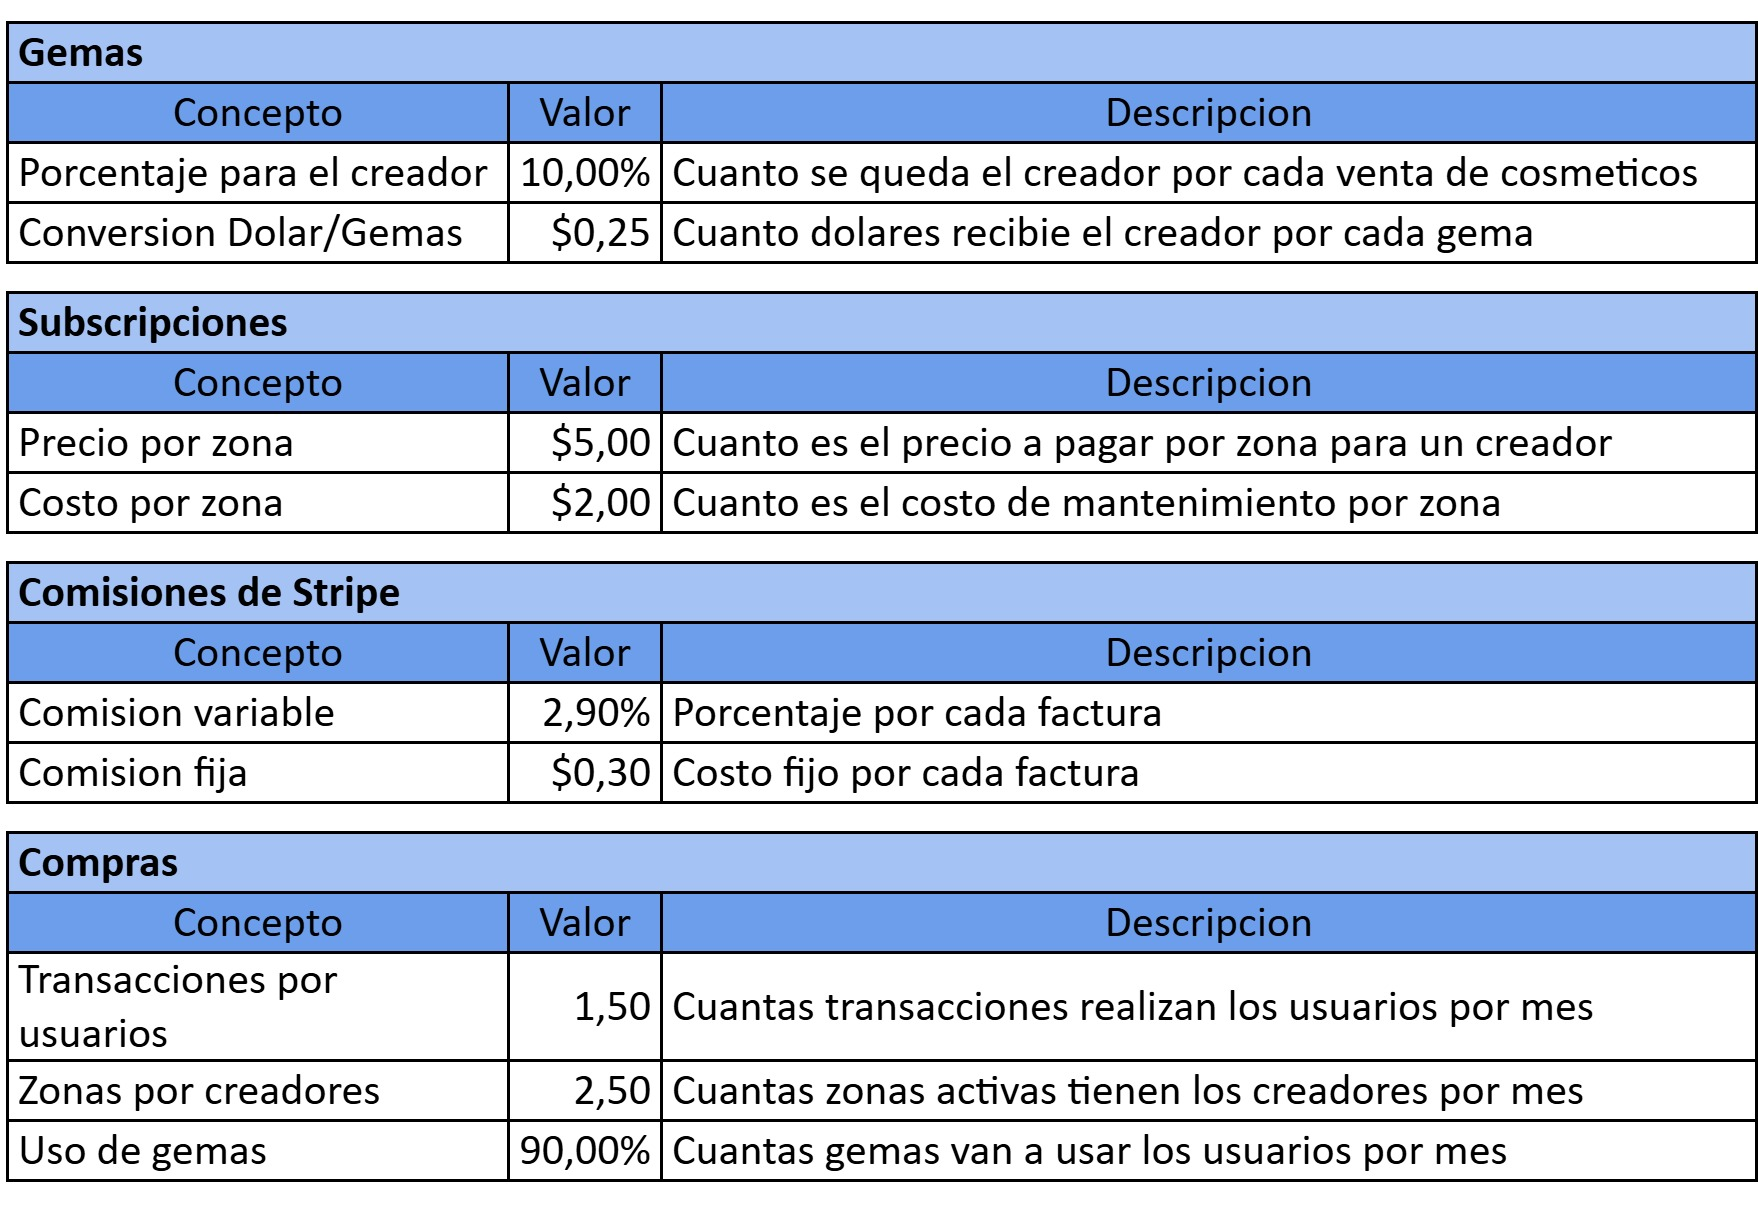
\includegraphics[width=0.65\textwidth]{img/08-implemented-solution/economy/assumptions.jpg}
  \caption{Resumen de los supuestos del modelo económico}
  \label{fig:assumptions}
\end{figure}

En cuanto a los packs de gemas disponibles, el \textit{Small Pack} (\$1{,}99 por gema) 
concentra el 98\% de las transacciones, lo que eleva el valor promedio por transacción 
a \$2{,}35 y la cantidad promedio de gemas adquiridas a 1{,}58 por compra.
\vspace{0.25cm}

\begin{figure}[H]
  \centering
  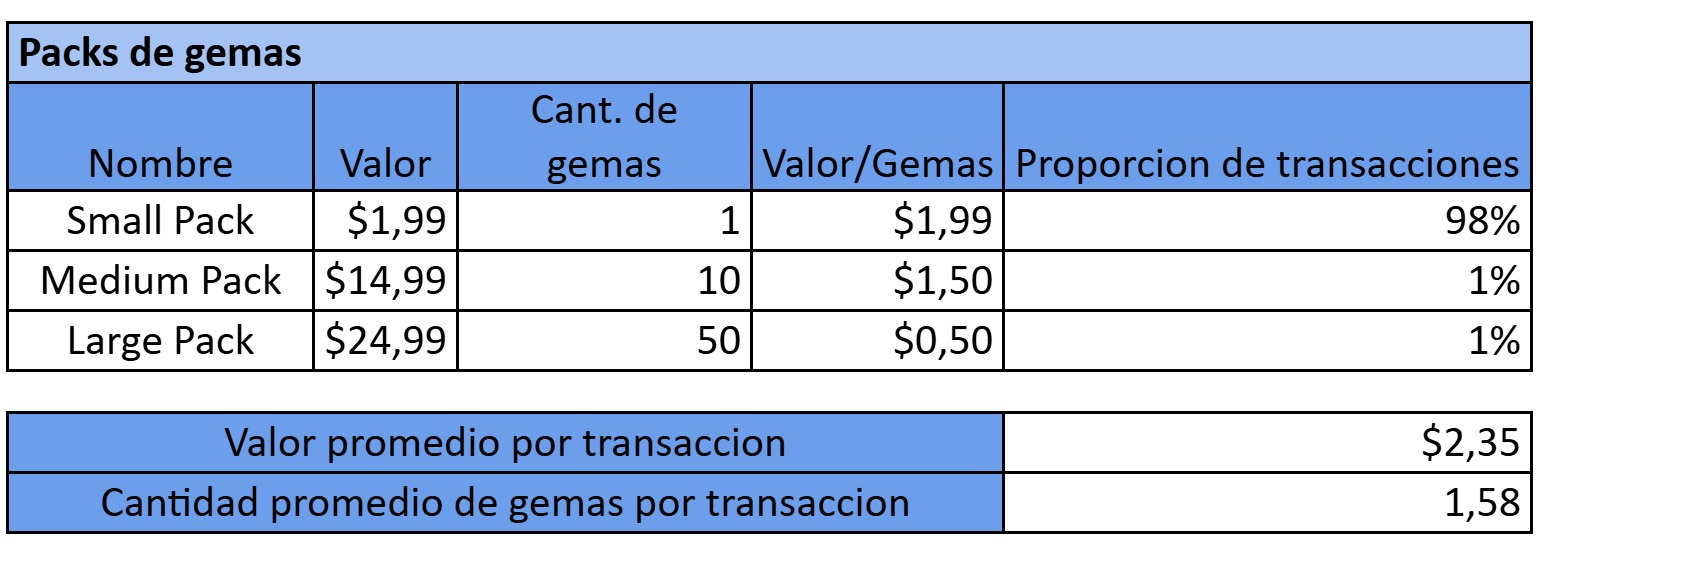
\includegraphics[width=0.65\textwidth]{img/08-implemented-solution/economy/gems-packs.jpg}
  \caption{Packs de gemas y su distribución en las transacciones}
  \label{fig:gems}
\end{figure}

\paragraph{Proyecciones de crecimiento}

Se modelaron cinco escenarios de crecimiento para usuarios y creadores a lo largo 
de 12 meses, con distintas tasas mensuales y bases iniciales:

\begin{itemize}
  \item \textbf{Pesimista:} crecimiento mensual del 2\% para usuarios (base: 5) 
  y del 1\% para creadores (base: 1), representando un crecimiento lento 
  pero sostenido.
  \item \textbf{Base:} tasas del 4\% y 3\% respectivamente, con bases de 10 
  usuarios y 1 creador, bajo un crecimiento moderado.
  \item \textbf{Optimista:} tasas del 8\% y 7\%, partiendo de 50 usuarios y 
  5 creadores, reflejando una adopción acelerada.
  \item \textbf{Arranque Lento:} crecimiento inicialmente bajo que se acelera 
  a partir del quinto mes, partiendo de 25 usuarios y 3 creadores.
  \item \textbf{Lanzamiento:} pico inicial fuerte (20\% en el primer mes) 
  seguido de una desaceleración progresiva, con bases de 150 usuarios y 
  15 creadores.
\end{itemize}

\begin{figure}[H]
  \centering
  \begin{adjustbox}{width=1.10\textwidth, center}
    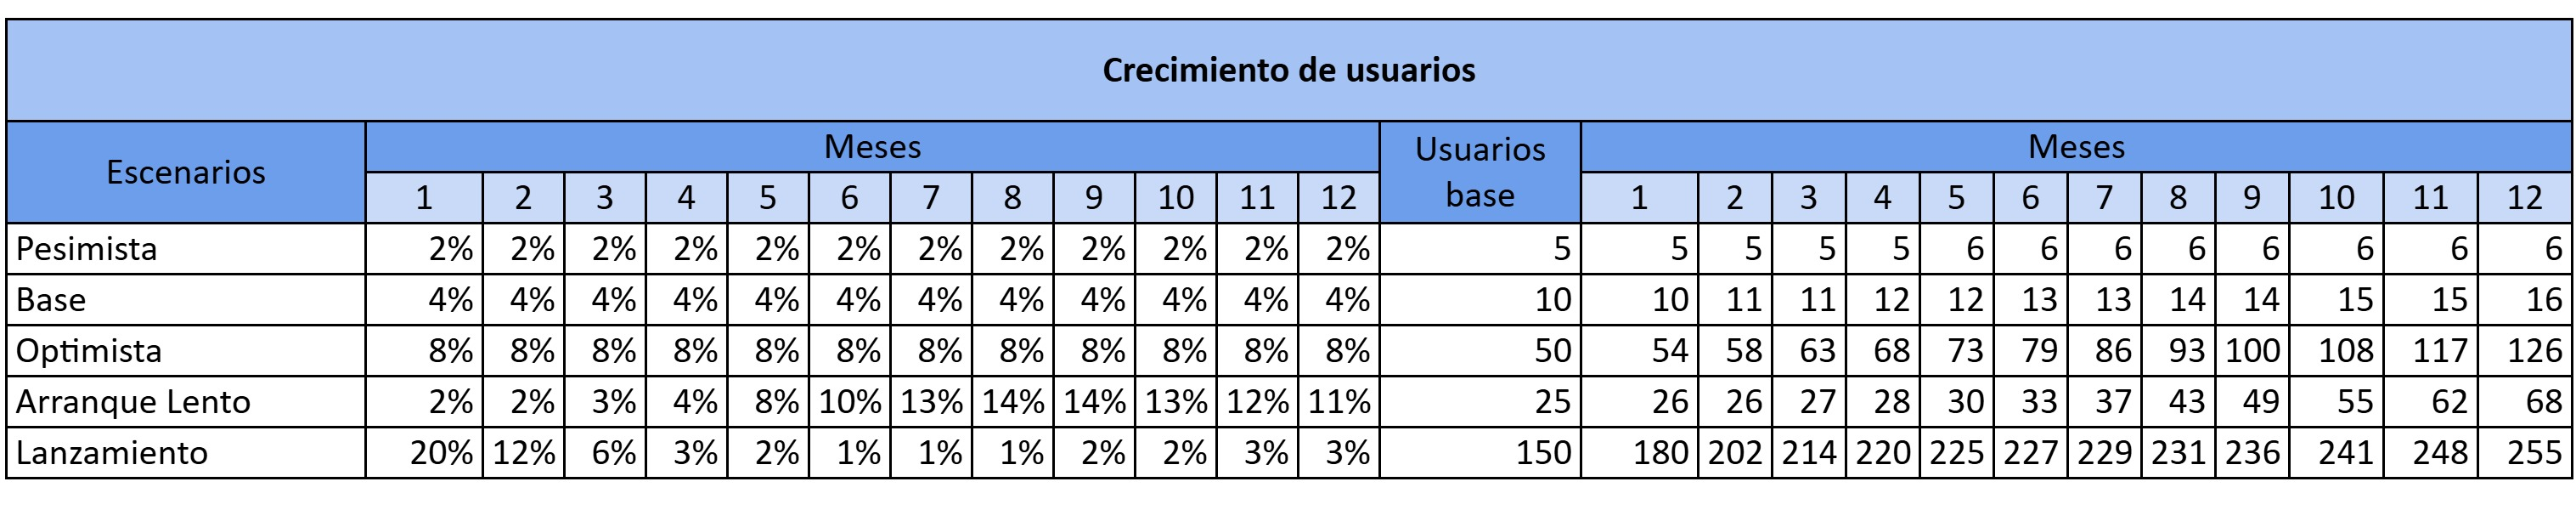
\includegraphics{img/08-implemented-solution/economy/users-scenarios.jpg}
  \end{adjustbox}
  \caption{Escenarios de crecimiento para usuarios}
  \label{fig:users-scenarios}
\end{figure}

\begin{figure}[H]
  \centering
  \begin{adjustbox}{width=1.10\textwidth, center}
    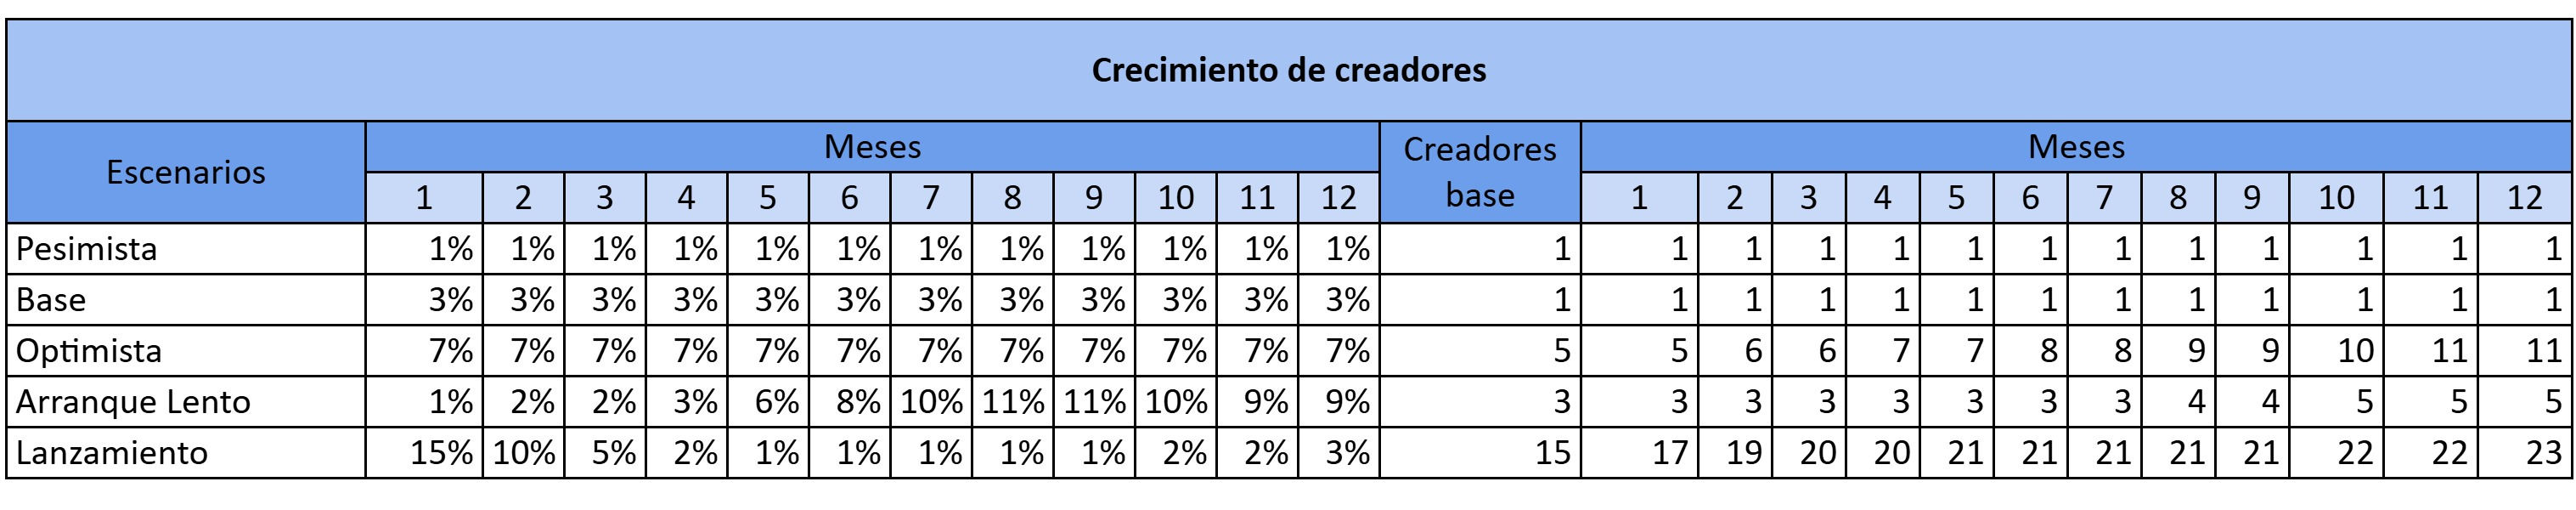
\includegraphics{img/08-implemented-solution/economy/creators-scenarios.jpg}
  \end{adjustbox}
  \caption{Escenarios de crecimiento para creadores}
  \label{fig:creators-scenarios}
\end{figure}

En cada uno de esos escenarios, se proyectaron los ingresos mensuales provenientes de las ventas de gemas y las suscripciones,
teniendo en cuenta los supuestos establecidos y todos los costos asociados, como las comisiones de Stripe y el mantenimiento de servidores.
A continuación, se presentan los resultados de cada escenario, destancando la rentabilidad a lo largo del tiempo.
\vspace{0.25cm}

\begin{figure}[H]
  \centering
  \begin{adjustbox}{width=1.10\textwidth, center}
    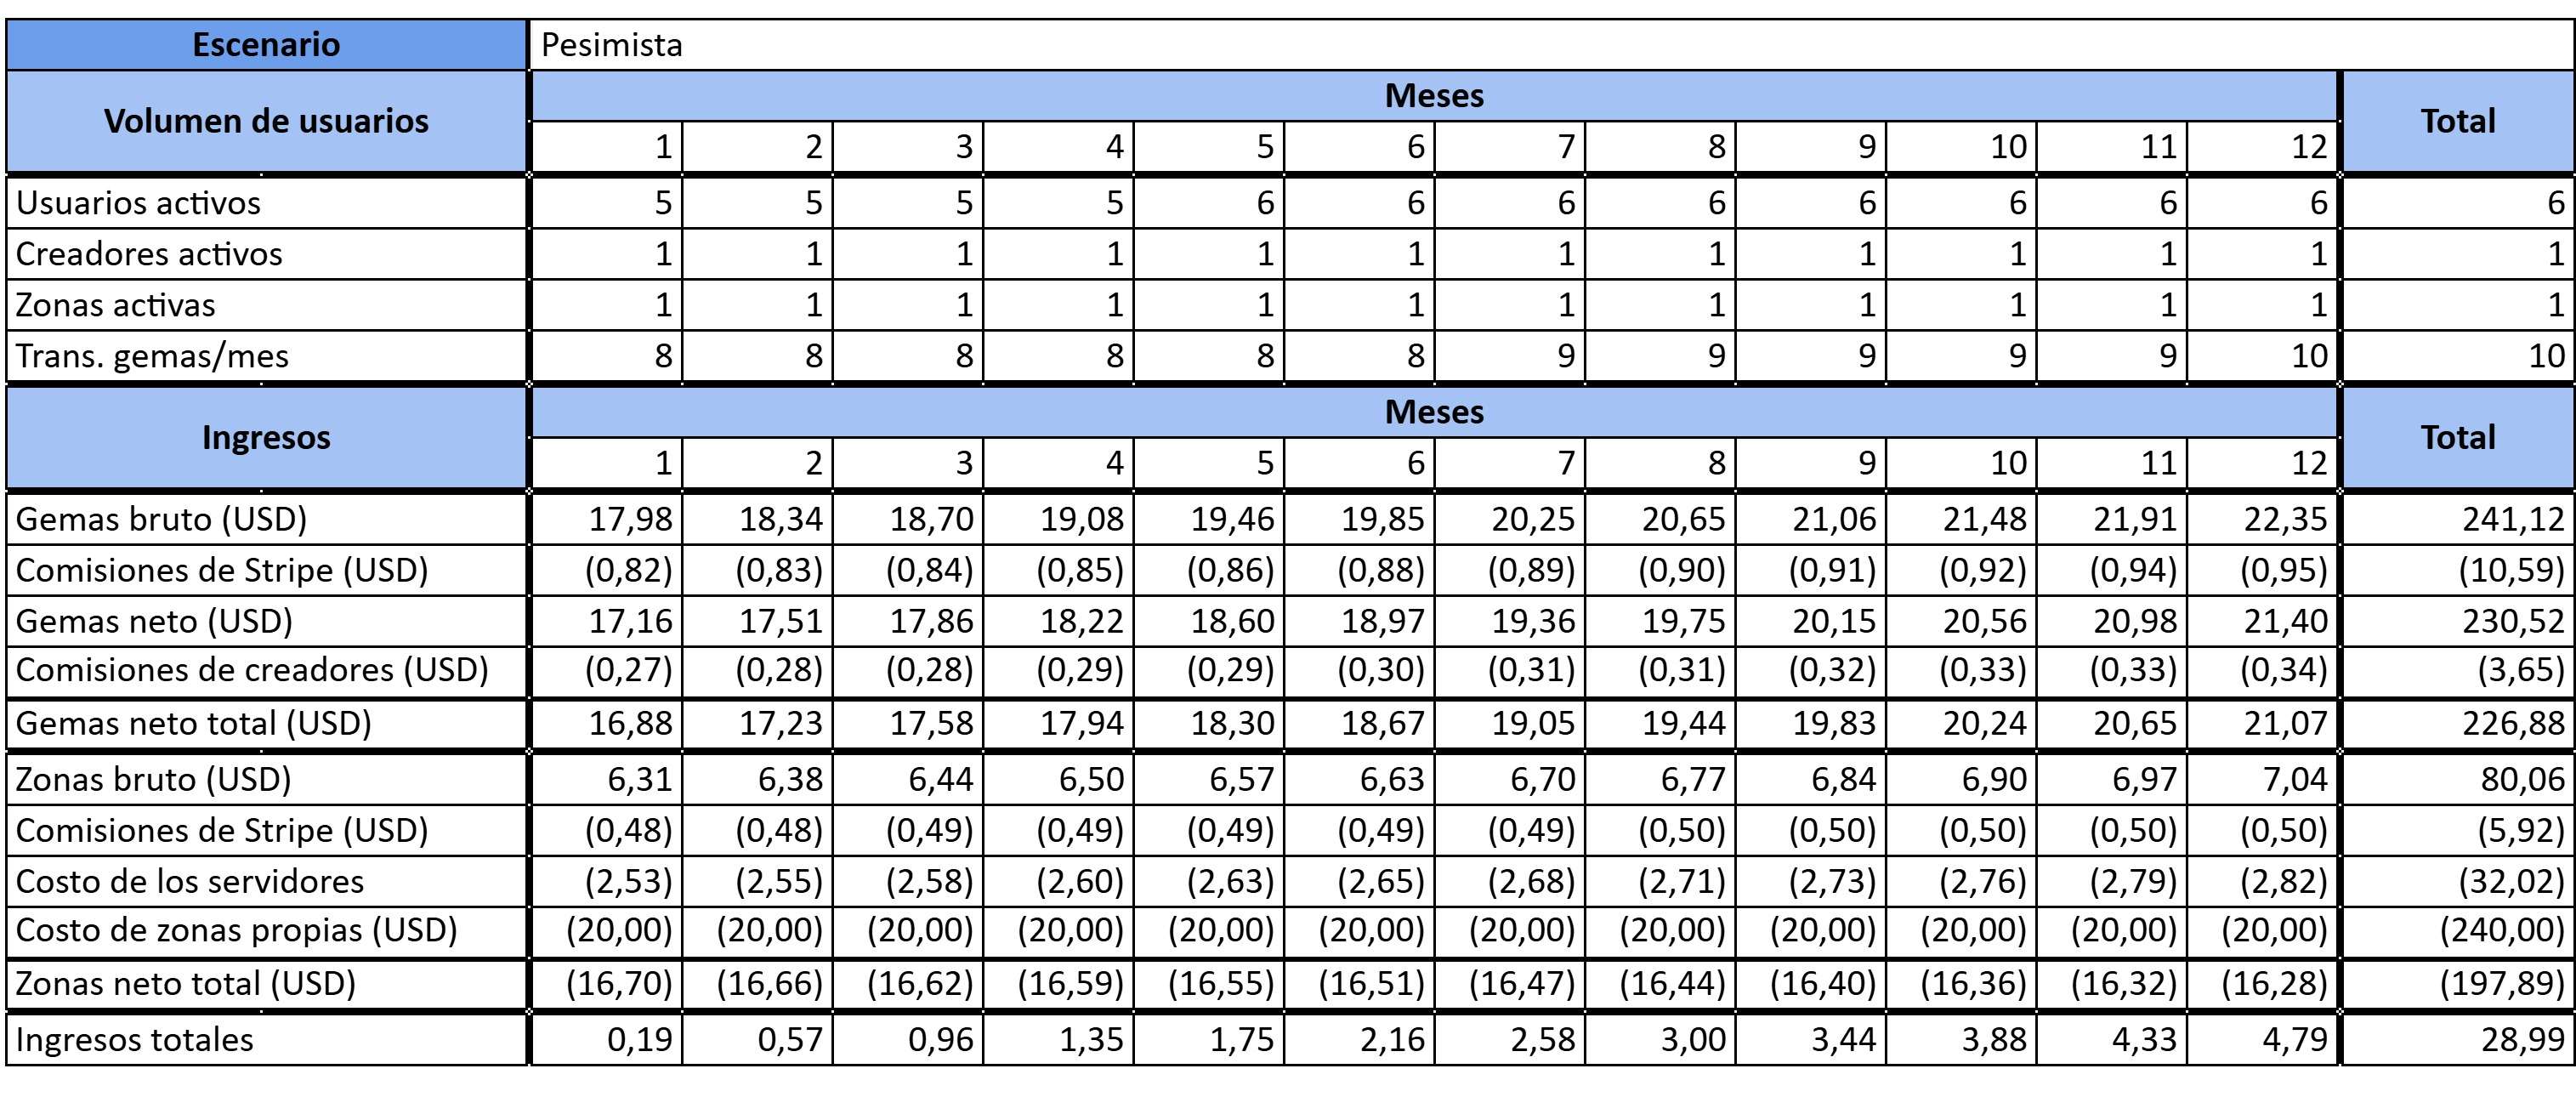
\includegraphics{img/08-implemented-solution/economy/scenarios/scenario-1.jpg}
  \end{adjustbox}
  \caption{Proyección de ingresos: Escenario Pesimista}
  \label{fig:scenarios-1}
\end{figure}

\begin{figure}[H]
  \centering
  \begin{adjustbox}{width=1.10\textwidth, center}
    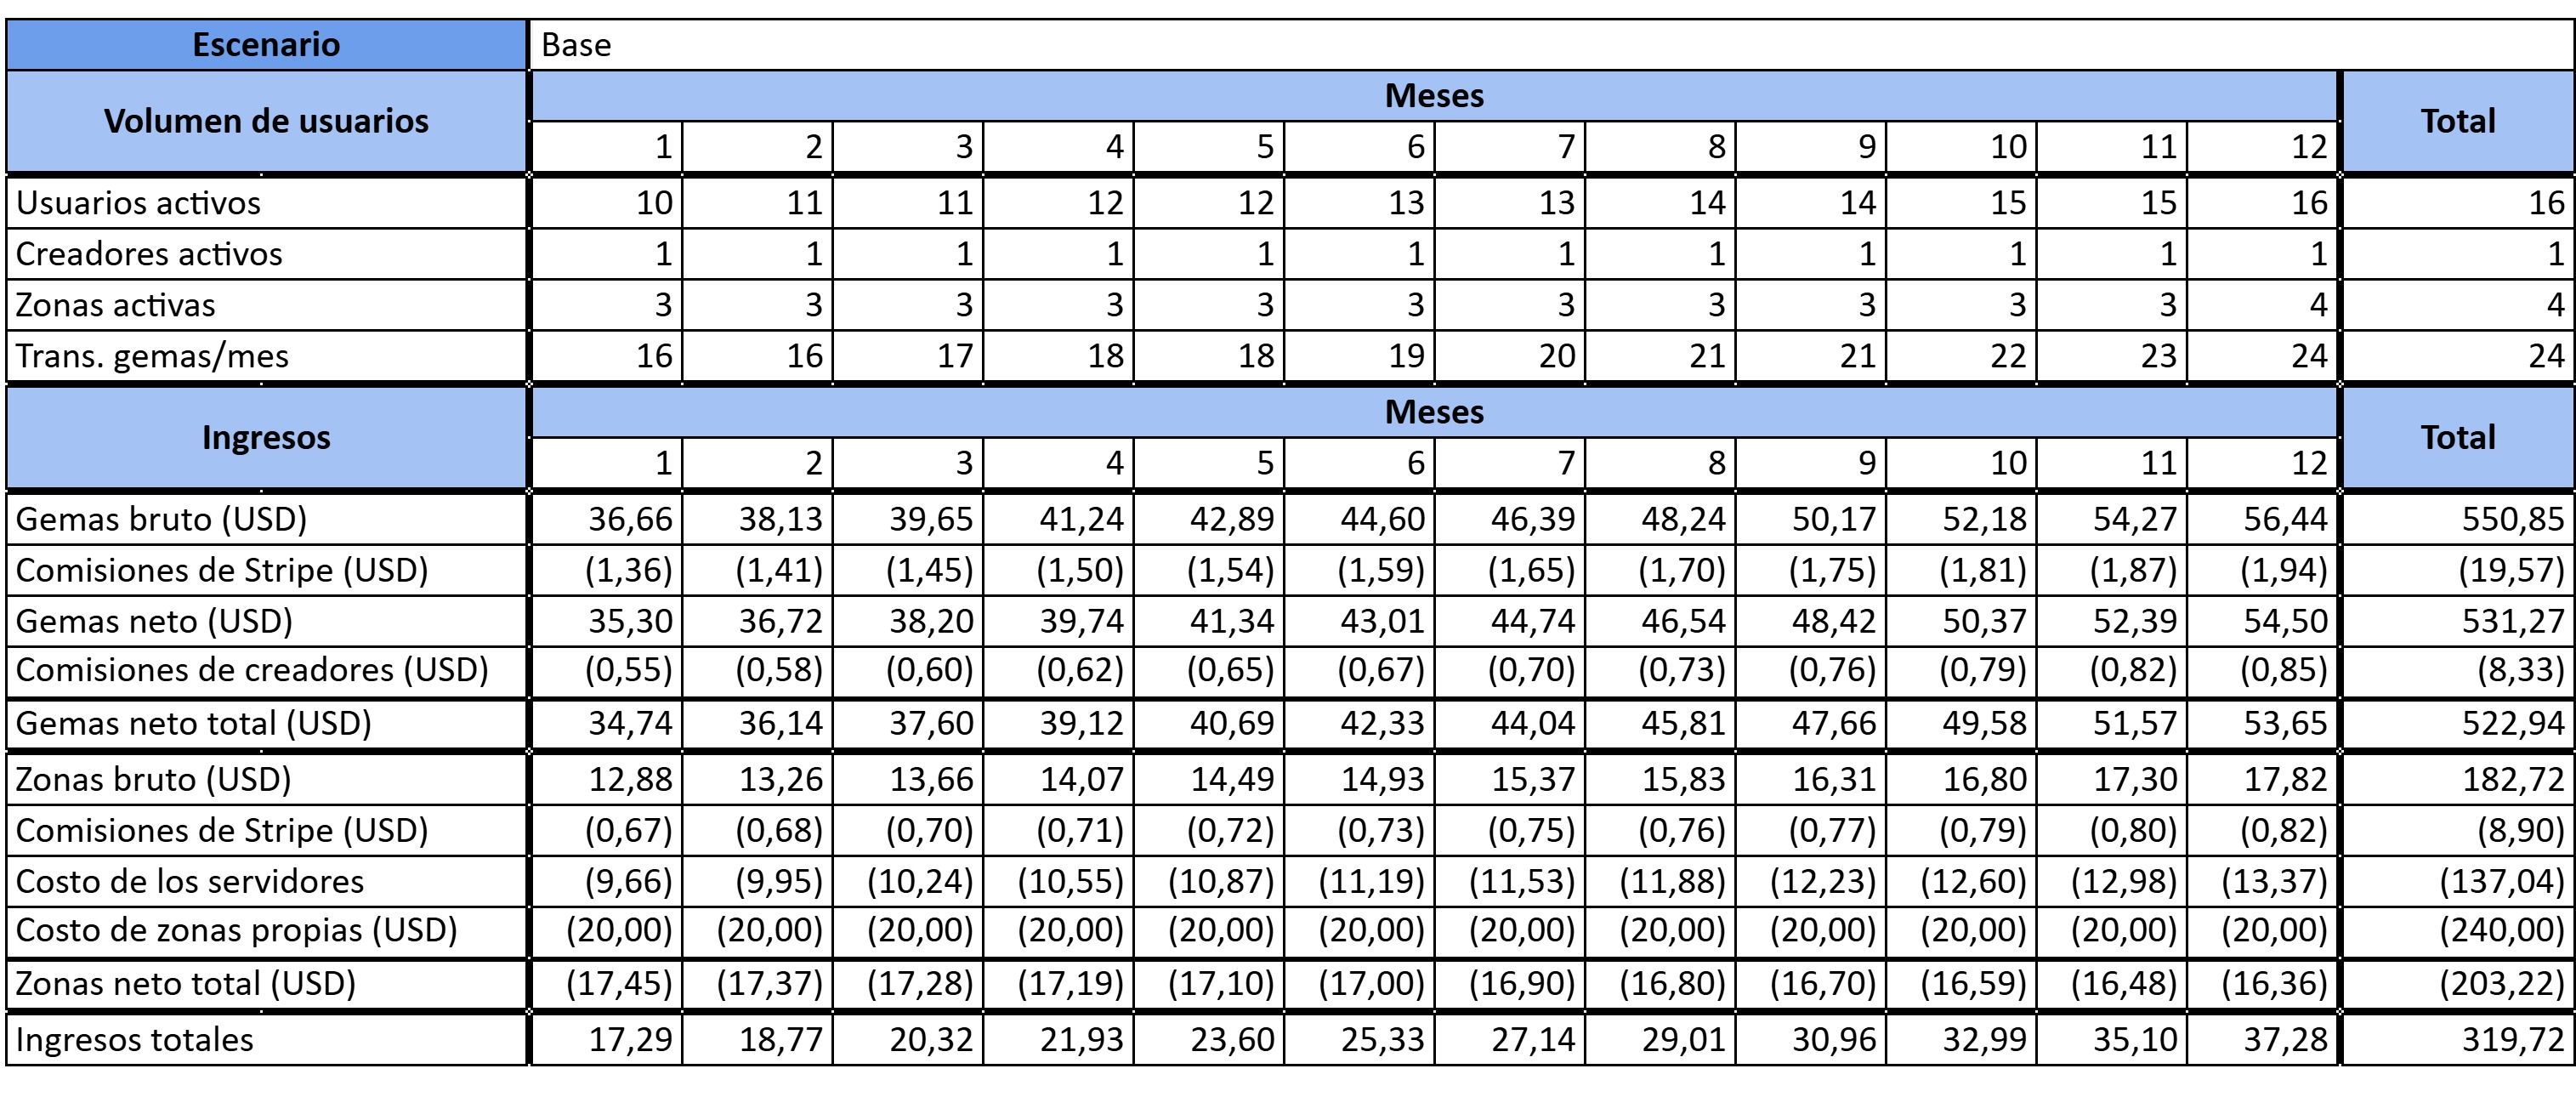
\includegraphics{img/08-implemented-solution/economy/scenarios/scenario-2.jpg}
  \end{adjustbox}
  \caption{Proyección de ingresos: Escenario Base}
  \label{fig:scenarios-2}
\end{figure}

\begin{figure}[H]
  \centering
  \begin{adjustbox}{width=1.10\textwidth, center}
    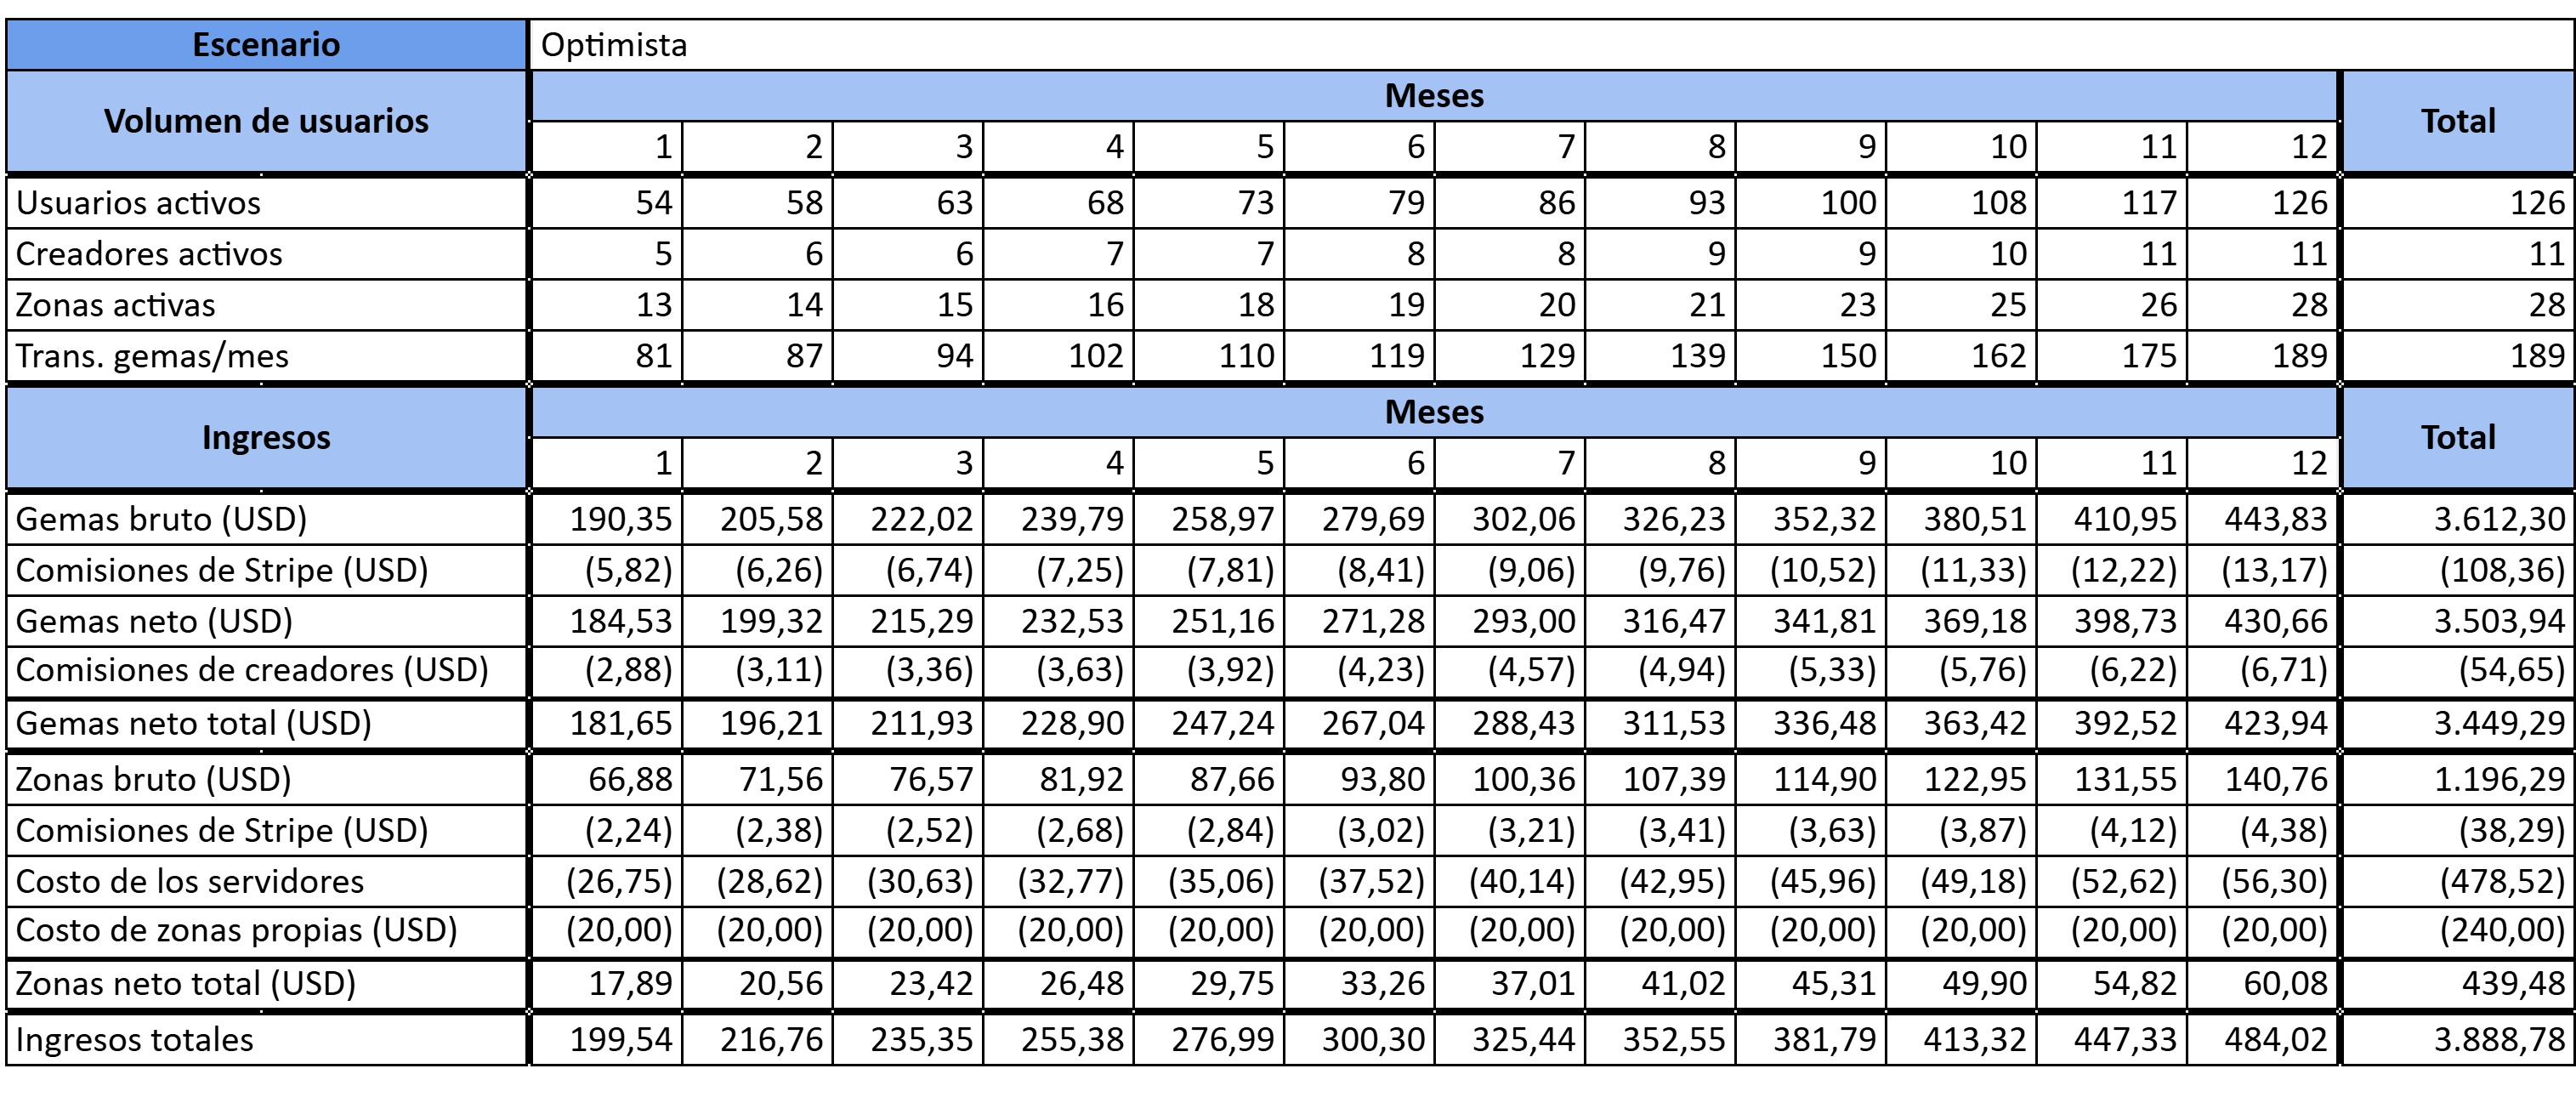
\includegraphics{img/08-implemented-solution/economy/scenarios/scenario-3.jpg}
  \end{adjustbox}
  \caption{Proyección de ingresos: Escenario Optimista}
  \label{fig:scenarios-3}
\end{figure}

\begin{figure}[H]
  \centering
  \begin{adjustbox}{width=1.10\textwidth, center}
    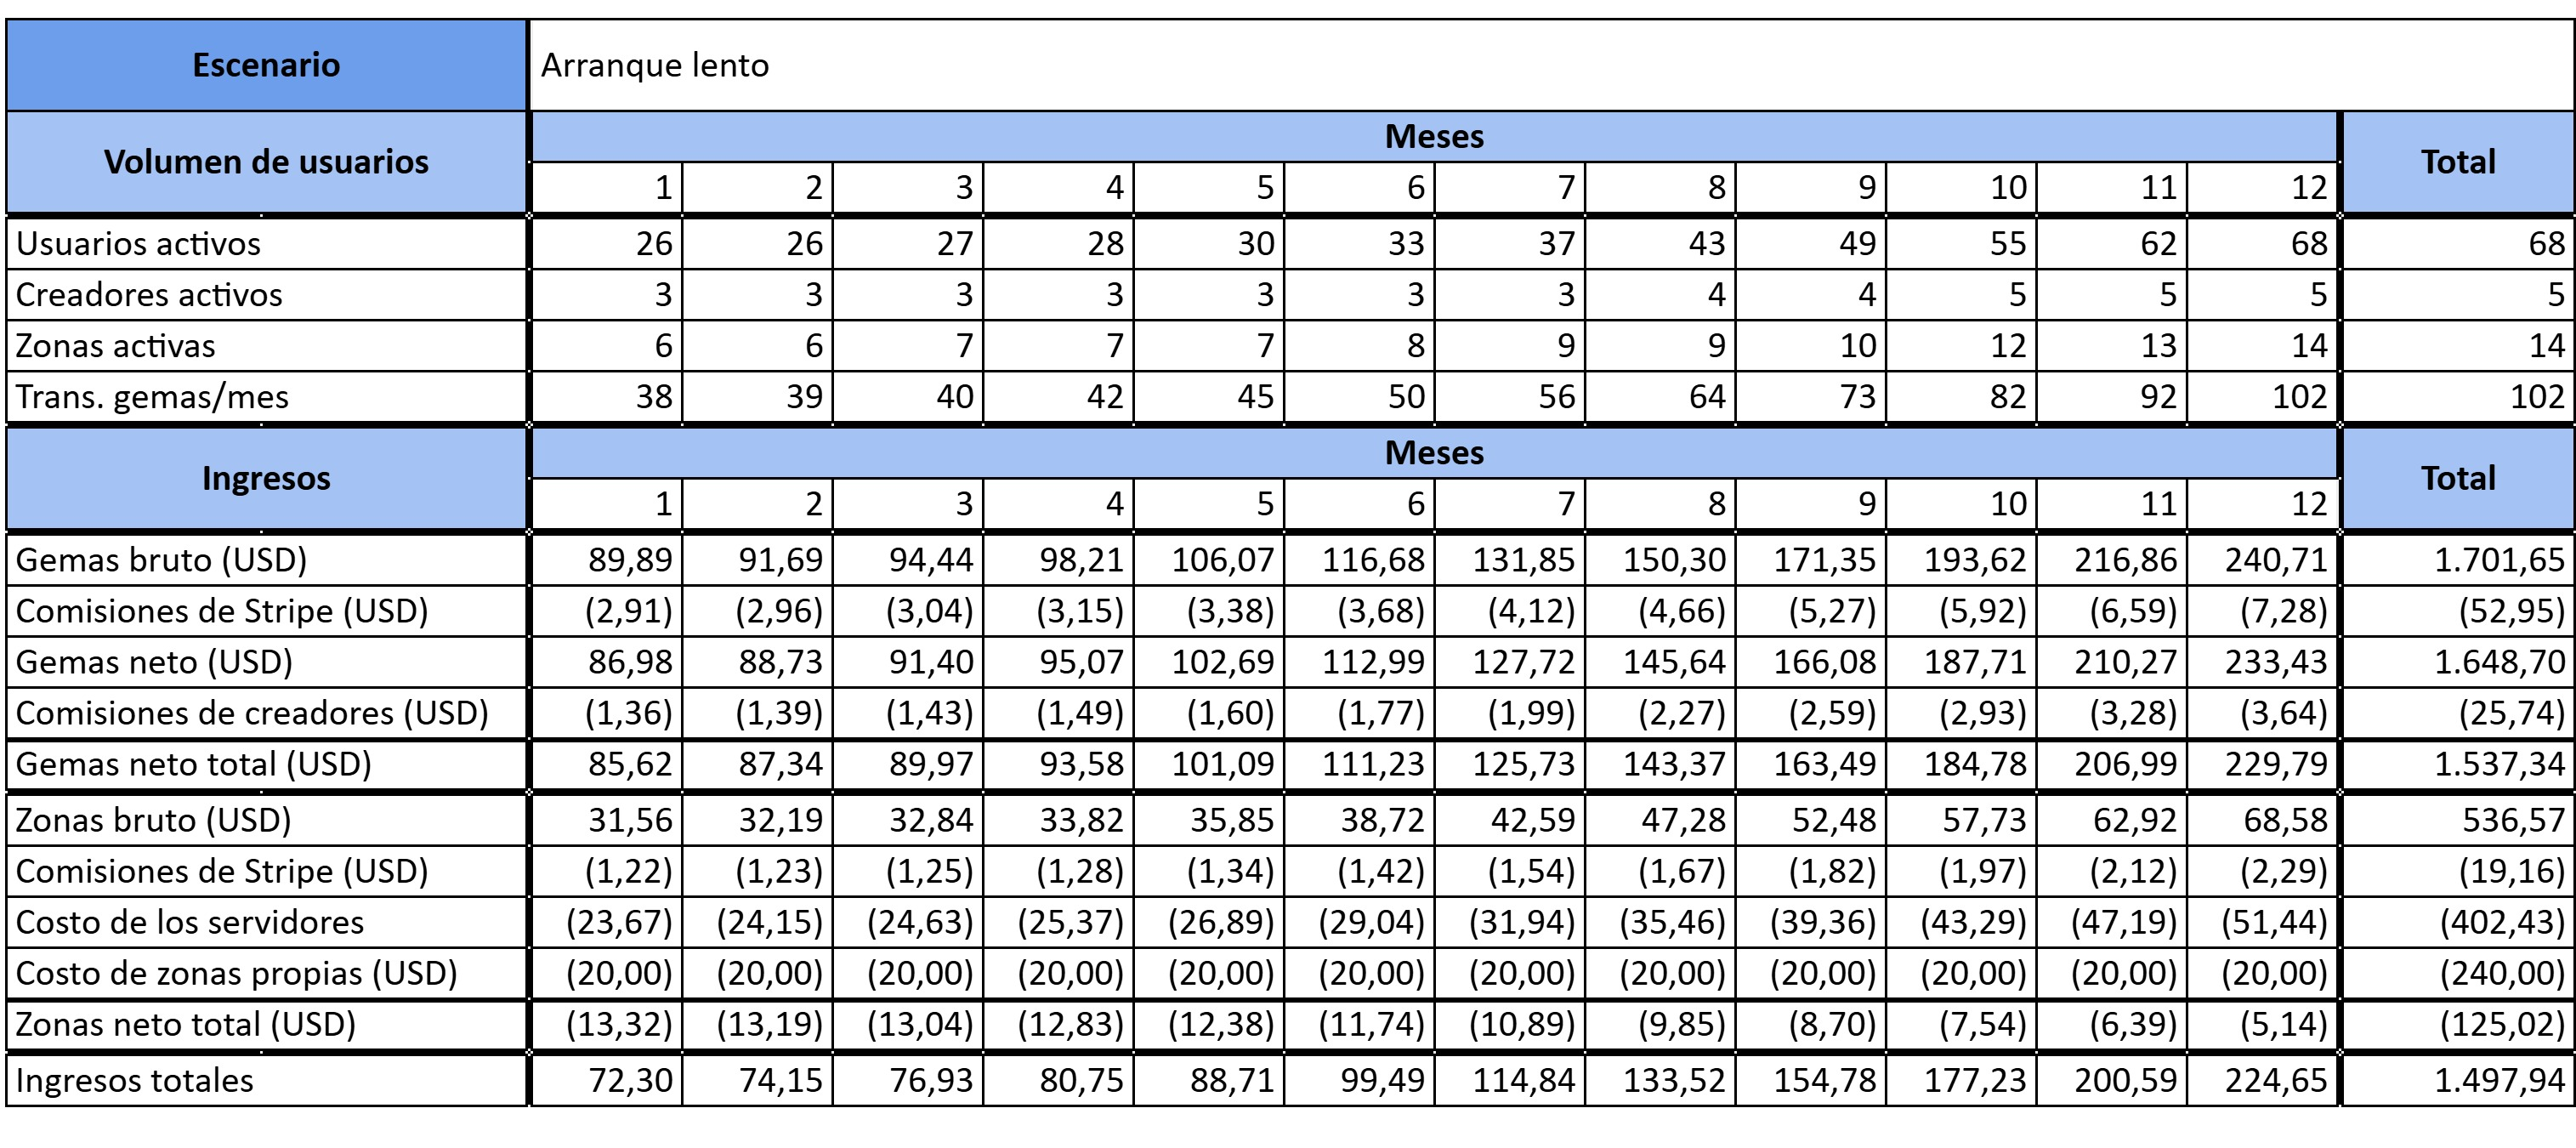
\includegraphics{img/08-implemented-solution/economy/scenarios/scenario-4.jpg}
  \end{adjustbox}
  \caption{Proyección de ingresos: Escenario Arranque Lento}
  \label{fig:scenarios-4}
\end{figure}

\begin{figure}[H]
  \centering
  \begin{adjustbox}{width=1.10\textwidth, center}
    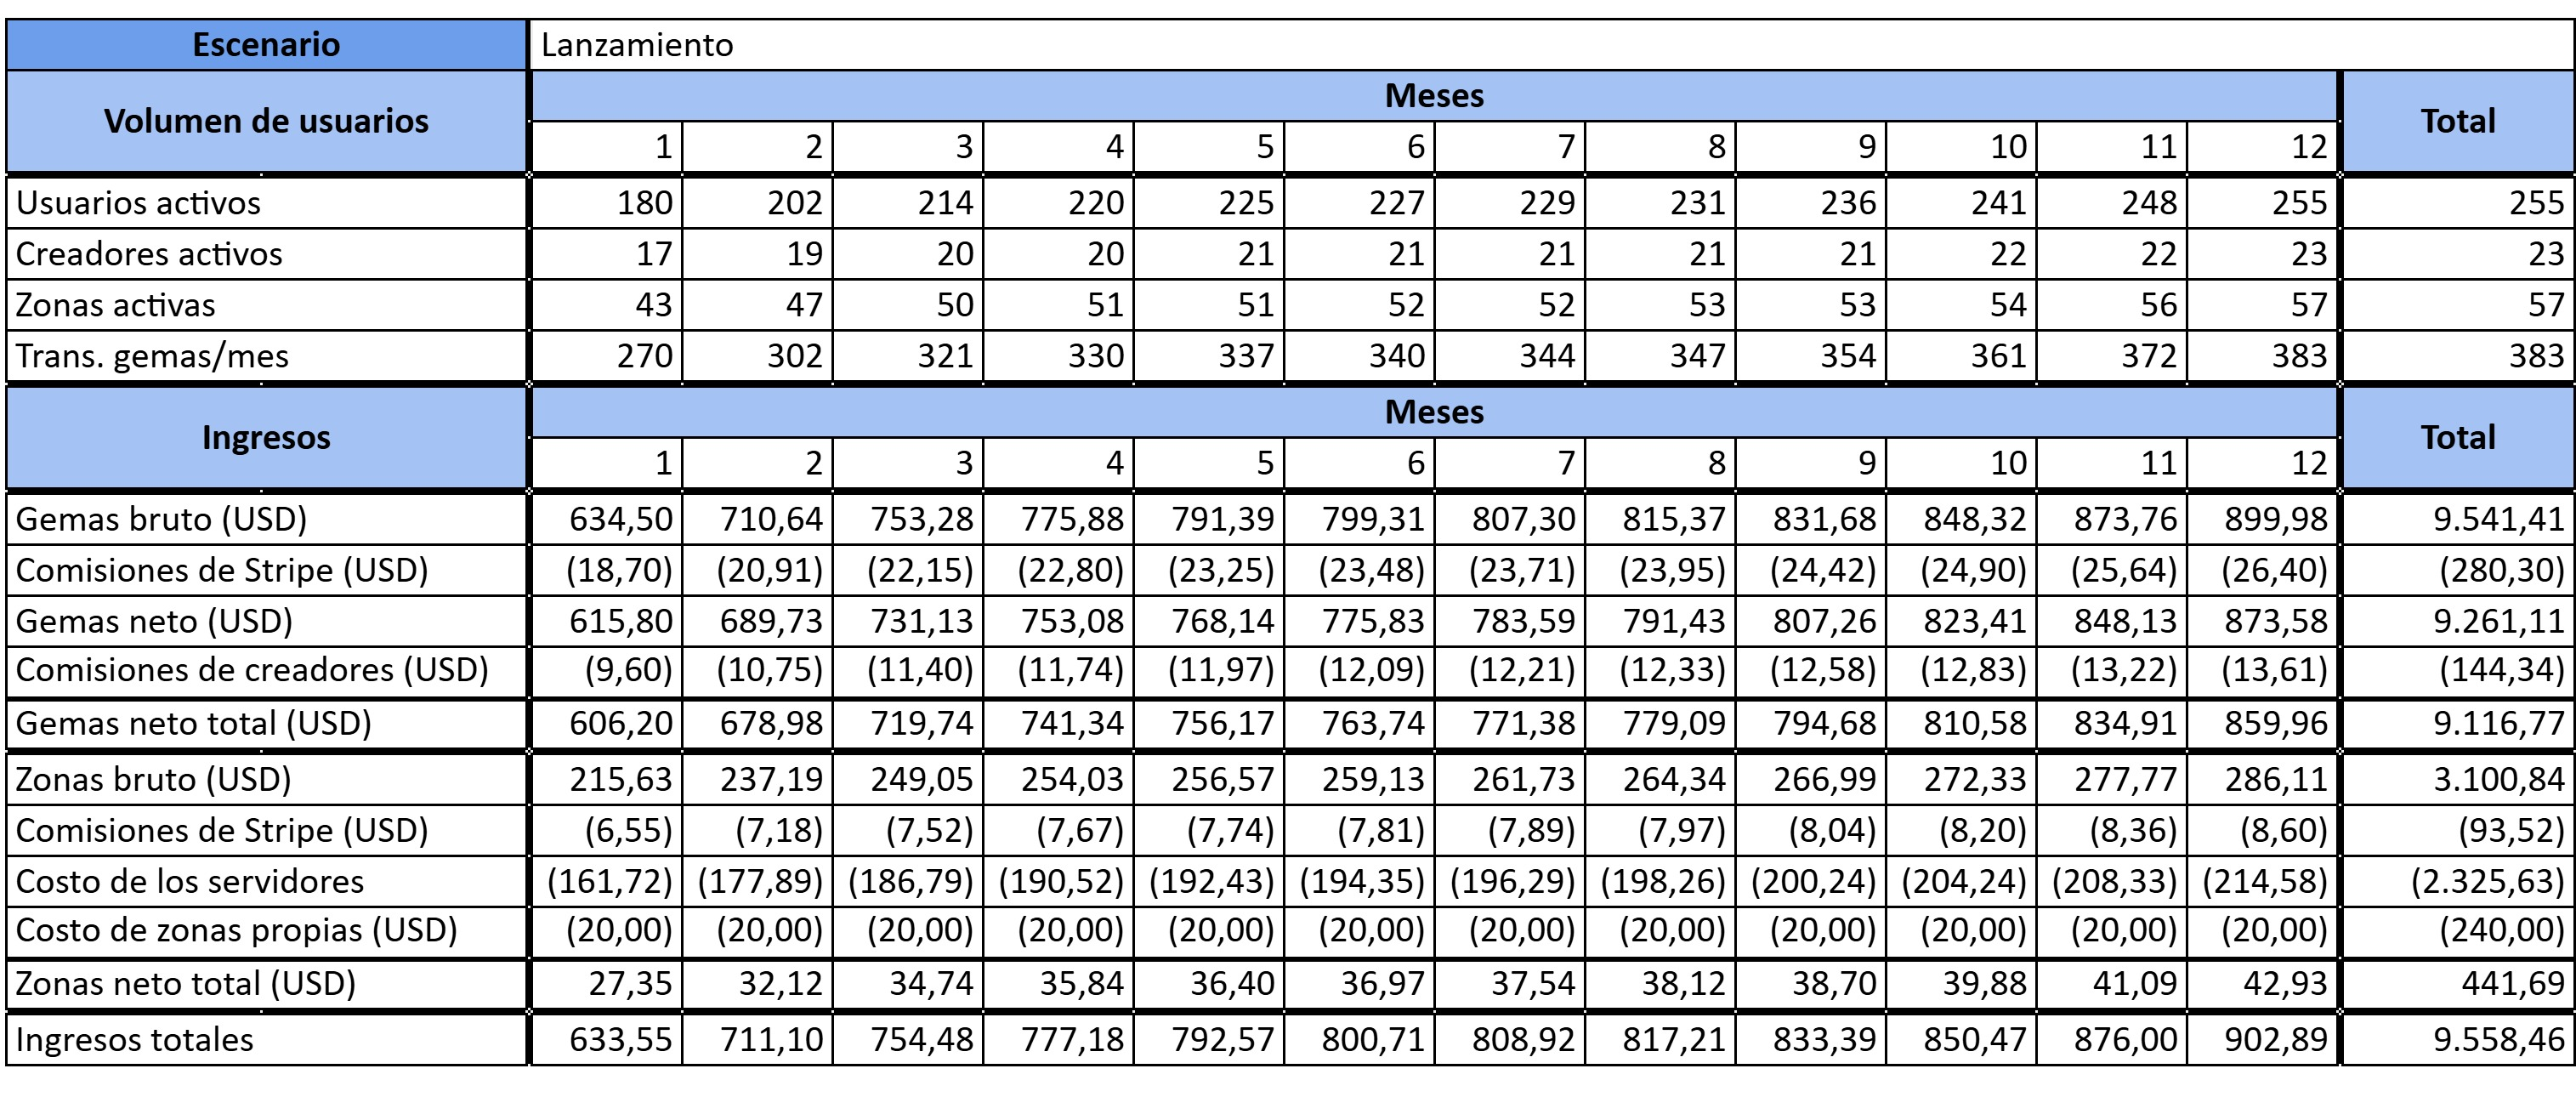
\includegraphics{img/08-implemented-solution/economy/scenarios/scenario-5.jpg}
  \end{adjustbox}
  \caption{Proyección de ingresos: Escenario Lanzamiento}
  \label{fig:scenarios-5}
\end{figure}
